\documentclass{article}
\usepackage{graphicx} % Required for inserting images
\usepackage[margin=2cm]{geometry} % Adjust the margins
\usepackage{amsmath}
\usepackage{amssymb}
\numberwithin{equation}{subsection}
\usepackage{float}

\title{MDCS Notes}
\author{Gregorio Valenti}
\date{}


\begin{document}

	\section{Feedback Control System Definition}
	\hspace{1cm}
	For this course, we will consider the model below to represent the system under study:
	
	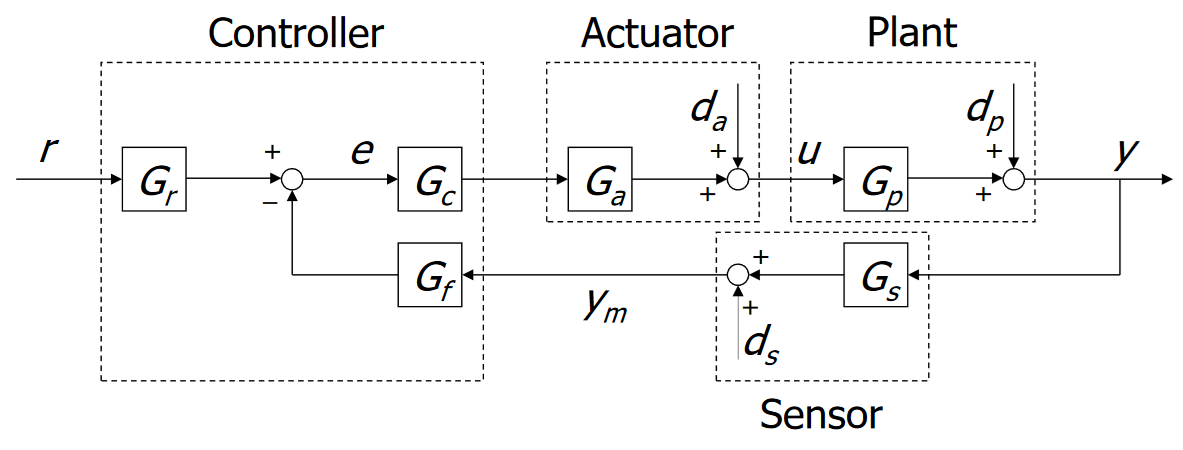
\includegraphics[scale=1]{images/feedback_loop_description.png}

	With the following characteristics:
	\begin{enumerate}
		\item[$\bullet$] Plant $G_p$ with disturbance $d_p$
		\item[$\bullet$] Actuator $G_a$ with disturbance $d_a$
		\item[$\bullet$] Sensor $G_s$ with disturbance $d_s$
		\item[$\bullet$] Feedback Controller $G_c$ 	
	\end{enumerate}
	
	\section{Step response of prototype $\boldmath{2}^{\textbf{nd}}$ order system}
	For a prototype second order system with Sensitivity and Complementary sensitivity functions of the form:
	\begin{equation}
		T(s) = \dfrac{1}{1+\dfrac{2\zeta}{\omega_n}s+\dfrac{s^2}{\omega_n^2}} \quad ; \quad S(s) = \dfrac{s\left(\dfrac{2\zeta}{\omega_n}+\dfrac{s}{\omega_n^2}\right)}{1+\dfrac{2\zeta}{\omega_n}s+\dfrac{s^2}{\omega_n^2}}
	\end{equation}
	
	
	From the transient response indices for maximum overshoot $\hat{s}$, rise time $t_r$ and settling time $t_{s,\alpha\%}$, we can compute the system's damping coefficient, as well as constraints on the natural frequency and resonance peaks $T_p$ and $S_p$:
	\begin{enumerate}
		\item[$\bullet$] $\displaystyle \zeta = \frac{\left| \log (\hat{s}) \right|}{\sqrt{\pi^2 + \log^2 (\hat{s})}} \hfill (2.0.2)$
		\item[$\bullet$] $\displaystyle \omega_{n,tr} = \frac{1}{t_r\sqrt{1-\zeta^2}} \cdot (\pi - acos(\zeta)) \quad; \quad
		\omega_{n,t,s\alpha \%} = \frac{\log(\frac{100}{\alpha})}{t_{s,\alpha \%}\zeta} \hfill (2.0.3)$
		\item[$\bullet$] $\displaystyle T_p = \frac{1}{2\zeta \sqrt{1-\zeta^2}} \quad; \quad S_p = \frac{2\zeta \sqrt{2+4\zeta^2+2\sqrt{1+8\zeta^2}}}{\sqrt{1+8\zeta^2}+4\zeta^2-1} \hfill (2.0.4)$
	\end{enumerate}
	
	\section{Steady-state Response to Polynomial Reference Inputs}
	Requirements on steady-state tracking error and steady-state errors in the presence of polynomial disturbances can be translated into constraints on the Sensitivity function.
	Therefore, by first writing $S(s) = s^{\nu+p}S^*(s)$, we can apply the final value theorem to each expression as described in the following subsections.
	\subsection{Tracking Error}
	\subsubsection{Problem formulation}
	The tracking error is defined as:
	\begin{equation}
		e_r(t) = y_d(t)-y_r(t) = K_dr(t)-y_r(t)
	\end{equation}
	Applying the final value theorem leads to:
	\begin{align}
		\left| e_r^\infty \right| &= \displaystyle\lim_{t\to\infty} 	\left|e_r(t)\right| = \displaystyle\lim_{s\to0}s \left|e_r(s)\right| = \displaystyle\lim_{s\to0}s \left|K_dr(s)-y_r(s)\right| = \nonumber \\
		&= \displaystyle\lim_{s\to0}s \left|G_{re}(s)r(s)\right| = 	\displaystyle\lim_{s\to0}s \left|S(s)K_dr(s)\right| = \nonumber \\
		&= \displaystyle\lim_{s\to0}s 	\left|s^{\nu+p}S^*(s)K_d\dfrac{R_0}{s^{h+1}}\right| =
		\begin{cases}
			0, & \text{if } \nu+p>h \\
			\left|S^*(0)K_dR_0\right|, & \text{if } \nu+p = h
		\end{cases}
	\end{align}
	The given system type is then $\nu+p$.
	\subsubsection{Conclusions}
	Considering the specification $\left|e_r^\infty\right| \leq \rho_r  $, we obtain the following result:
	\begin{enumerate}
		\item[$\bullet$] case $\rho_r=0 \implies S(s)$ must have a zero at $s=0$ with multiplicity greater than $h \implies$ We have no constraint on $\left|S^*(0)\right| $ 
		\item[$\bullet$] case $\rho_r>0 \implies S(s)$ must have a zero at $s=0$ with multiplicity $h \implies$ We have the following constraint:
		\begin{equation}
			\left|S^*(0)\right| \leq \dfrac{\rho_r}{K_dR_0}	
		\end{equation}
	\end{enumerate}
	
	\subsection{Error due to Generic Polynomial Disturbances $\boldsymbol{d(t)}$}
	\subsubsection{Problem formulation}
	The output error due to the generic disturbance $d(t)$ is the contribution of the disturbance to the output $y(t)$:
	\begin{equation}
		e_d(t) = y_d(t)
	\end{equation}
	
	\subsubsection{Polynomial disturbance $\boldsymbol{d_a(t)}$}
	Applying the final value theorem leads to:
	\begin{align}
		\left| e_{d_a}^\infty \right| &= \displaystyle\lim_{t\to\infty} 	\left|e_{d_a}(t)\right| = \displaystyle\lim_{s\to0}s \left|e_{d_a}(s)\right| = \displaystyle\lim_{s\to0}s \left|y_{d_a}(s)\right| = \displaystyle\lim_{s\to0}s \left| S(s)G_p(s)d_a(s) \right| = \nonumber \\
		&= \displaystyle\lim_{s\to0} 	\left|s^{\nu+p+1}S^*(s)G_p(s)\dfrac{D_{a0}}{s^{h+1}}\right| = \displaystyle\lim_{s\to0} \left|s^{\nu+1}S^*(s)K_p\dfrac{D_{a0}}{s^{h+1}}\right| =
		\begin{cases}
			0, & \text{if } \nu>h \\
			\left|S^*(0)K_pD_{a0}\right|, & \text{if } \nu = h
		\end{cases}
	\end{align}
	We then obtain two cases as before:
	\begin{enumerate}
		\item[$\bullet$] case $\rho_a=0 \implies S(s)$ must have a zero at $s=0$ with multiplicity greater than $h \implies$ We have no constraint on $\left|S^*(0)\right| $ 
		\item[$\bullet$] case $\rho_a>0 \implies S(s)$ must have a zero at $s=0$ with multiplicity $h \implies$ We have the following constraint:
		\begin{equation}
			\left|S^*(0)\right| \leq \dfrac{\rho_a}{K_pD_{a0}}	
		\end{equation}
	\end{enumerate}
	
	\subsubsection{Polynomial disturbance $\boldsymbol{d_p(t)}$}
	Applying the final value theorem leads to:
	\begin{align}
		\left| e_{d_p}^\infty \right| &= \displaystyle\lim_{t\to\infty} 	\left|e_{d_p}(t)\right| = \displaystyle\lim_{s\to0}s \left|e_{d_p}(s)\right| = \displaystyle\lim_{s\to0}s \left|y_{d_p}(s)\right| = \displaystyle\lim_{s\to0}s \left| S(s)d_p(s) \right| = \nonumber \\
		&= \displaystyle\lim_{s\to0}	\left|s^{\nu+p+1}S^*(s)\dfrac{D_{p0}}{s^{h+1}}\right| =
		\begin{cases}
			0, & \text{if } \nu+p>h \\
			\left|S^*(0)D_{p0}\right|, & \text{if } \nu+p = h
		\end{cases}
	\end{align}
	We then obtain two cases as before:
	\begin{enumerate}
		\item[$\bullet$] case $\rho_p=0 \implies S(s)$ must have a zero at $s=0$ with multiplicity greater than $h \implies$ We have no constraint on $\left|S^*(0)\right| $ 
		\item[$\bullet$] case $\rho_p>0 \implies S(s)$ must have a zero at $s=0$ with multiplicity $h \implies$ We have the following constraint:
		\begin{equation}
			\left|S^*(0)\right| \leq \dfrac{\rho_p}{D_{p0}}	
		\end{equation}
	\end{enumerate}
	
	\section{Steady-state Response to Sinusoidal Disturbances}
	\subsection{Output disturbance $\boldsymbol{d_p(t)}$}
	The focus is on the class of sinusoidal signals of the following type:
	\begin{equation}
		d_p = a_p\sin(\omega_pt) \quad \forall\omega_p\leq\omega_p^+ \quad \text{given } a_p \text{ and } w_p^+
	\end{equation}
	The output at steady-state is required to be bounded by a given constant:
	\begin{equation}
		\left| e_{d_p}^\infty \right| = \left| y_{d_p}^\infty \right| \leq \rho_p \quad \text{with } \rho_p>0
	\end{equation}
	The specification leads to a frequency domain constraint on the Sensitivity function $S(s)$ which can be computed as follows:
	\begin{align}
		\left| e_{d_p}^\infty \right| &= \left| y_{d_p}^\infty \right| = \left| a_pS(j\omega_p)\sin(\omega_pt+\varphi_p) \right| \leq a_p\left|S(j\omega_p)\right| \leq \rho_p \nonumber \\
		&\implies \left|S(j\omega_p)\right| \leq \dfrac{\rho_p}{a_p} = M_S^{LF} \quad \forall\omega_p \leq \omega_p^+
	\end{align}
	
	\subsection{Sensor Noise $\boldsymbol{d_s(t)}$}
	The focus is on the class of sinusoidal signals of the following type:
	\begin{equation}
		d_s = a_s\sin(\omega_st) \quad \forall\omega_s\geq\omega_s^- \quad \text{given } a_s \text{ and } w_s^-
	\end{equation}
	The output at steady-state is required to be bounded by a given constant:
	\begin{equation}
		\left| e_{d_s}^\infty \right| = \left| y_{d_s}^\infty \right| \leq \rho_s \quad \text{with } \rho_s>0
	\end{equation}
	The specification leads to a frequency domain constraint on the Complementary Sensitivity function $T(s)$ which can be computed as follows:
	\begin{align}
		\left| e_{d_s}^\infty \right| &= \left| y_{d_s}^\infty \right| = \left| a_sT(j\omega_s)\dfrac{1}{G_s}\sin(\omega_st+\varphi_s) \right| \leq a_s\left|T(j\omega_s)\dfrac{1}{G_s}\right| \leq \rho_s \nonumber \\
		&\implies \left|T(j\omega_s)\right| \leq \dfrac{\rho_sG_s}{a_s} = M_T^{HF} \quad \forall\omega_s \leq \omega_s^-
	\end{align}
	
	
	\section{Weighting Functions Construction}
	\subsection{Rational Approximation of Frequency Constraints}
	\begin{enumerate}
		\item[$\bullet$] Rational functions of the Laplace variable s are used to approximate the frequency domain constraints on $S(s)$ and $T(s)$.
		\item[$\bullet$] The parameters of the approximating functions (steady-state gain zeros and poles) can be moved to get the desired result.
		\item[$\bullet$] Butterworth polynomials can be used either as denominator or numerator of the approximating rational function to effectively retain constraints on different frequency ranges.
	\end{enumerate}
	\begin{table}[H] % Use [H] to fix position
		\begin{minipage}{0.45\textwidth} % Adjust width as needed
			\centering
			\begin{tabular}{|c|c|}
				\hline
				\textbf{Polynomial Order} & \textbf{Polynomial Structure} \\ \hline
				0 & $1$ \\ \hline
				1 & $1+\dfrac{s}{\omega_a}$ \\ \hline
				2 & $1+\dfrac{2\zeta}{\omega_a}s+\left(\dfrac{s}{\omega_a}\right)^2$ \\ \hline
				3 & $1+\dfrac{2}{\omega_a}s+2\left(\dfrac{s}{\omega_a}\right)^2+\left(\dfrac{s}{\omega_a}\right)^3$ \\ \hline
			\end{tabular}
			\caption{Butterworth Polynomials}
			\label{tab:polynomial_table}
		\end{minipage}
		\hfill
		\begin{minipage}{0.5\textwidth}
			\raggedright
			\vspace{-54pt}
			The key property of Butterworth polynomials is that, when used in the numerator or denominator of a rational function, they increase or decrease the frequency response magnitude by 3 dB respectively, at the frequency $\omega_a$, regardless of the polynomial's order.
		\end{minipage}
	\end{table}
	The goal is to obtain the rational functions $W_S^{-1}(s)$ and $W_T^{-1}(s)$ such that the constraints derived above are satisfied.
	\begin{enumerate}
		\item[$\bullet$] Considering low frequencies we have:
		\begin{equation}
			\left| W_S^{-1}(j\omega) \right| \leq M_S^{LF} \quad \forall 	\omega_p\leq\omega_p^+ \quad ; \quad \max_\omega \left| W_S^{-1}(\infty) \right| \leq S_{p0}
		\end{equation}	
		\item[$\bullet$] Considering high frequencies we have:
		\begin{equation}
			\left| W_T^{-1}(j\omega) \right| \leq M_T^{HF} \quad \forall 	\omega_s\geq\omega_s^- \quad ; \quad \max_\omega \left| W_T^{-1}(j\omega) \right| \leq T_{p0} \implies \left| W_T^{-1}(0) \right| = T_{p0}
		\end{equation}
	\end{enumerate}
	
	\section{Performance Specification as $\boldsymbol{H_\infty}$ Norm Constraints}
	\subsection{$\boldsymbol{H_\infty}$ Norm Definition}
	By defining:
	\begin{enumerate}
		\item[$\bullet$] $W_S(s)$ as the inverse of the rational approximation of the frequency domain constraints on the Sensitivity function S(s)
		\item[$\bullet$] $W_T(s)$ as the inverse of the rational approximation of the frequency domain constraints on the Complementary Sensitivity function T(s)
	\end{enumerate}
	Design constraints obtained from the considered performance requirements can be written in the following compact form:
	\begin{equation}
		\left| W_S(j\omega)S(j\omega) \right| \leq 1 \quad ; \quad \left| W_T(j\omega)T(j\omega) \right| \leq 1 \quad \forall\omega	
	\end{equation}
	The $H_\infty$ norm of a SISO LTI system with transfer function $H(s)$ is defined as:
	\begin{equation}
		\left\lVert H(s) \right\rVert_\infty \triangleq \max_\omega \left| H(j\omega) \right|
	\end{equation}
	It is now possible to rewrite the design constraints obtained above in terms of the weighted $H_\infty$ norm of $S(s)$ and $T(s)$:
	\begin{equation}
		\left\lVert W_S(s)S(s) \right\rVert_\infty \leq 1 \quad ; \quad \left\lVert W_T(s)T(s) \right\rVert_\infty \leq 1
	\end{equation}
	
	
\end{document}